%==========================================================================%
\documentclass[a4paper, 12pt]{article}

\usepackage{array}
\usepackage{amssymb}
%\usepackage{times}
\usepackage[spanish, activeacute]{babel}
\usepackage{graphicx}
\usepackage{hyperref}
%\usepackage[utf8]{inputenc}
\usepackage{fancyhdr}
\usepackage{xtab}
\usepackage{color}
\usepackage{lscape}
\usepackage{longtable}
\usepackage{tabularx}
\usepackage{fontspec}
\setsansfont{Roboto Condensed}
\usepackage{colortbl}
\usepackage{graphics}

\usepackage{cite}
\usepackage{lscape}
%\usepackage[T1]{fontenc}

\newenvironment{colortext}[1]{\color{#1}}{\ignorespacesafterend}

\renewcommand{\familydefault}{\sfdefault}







\pagestyle{fancyplain}

 \renewcommand{\sectionmark}[1]
                 {\markright{\thesection\ #1}}

 \newcommand{\coltex}[1]{\textcolor{red}{#1}}

                 
% \lhead[\fancyplain{}{\bfseries\thepage}]
%       {\fancyplain{}{\bfseries\rightmark}}
%
 \rhead[\fancyplain{}{\bfseries\leftmark}]{\fancyplain{}{\bfseries\thepage}}


 \setlength{\headheight}{34.43594pt}

 \lhead[\fancyplain{}{\vspace{-1cm}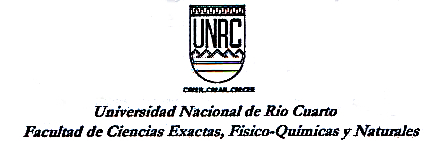
\includegraphics[scale=.4]{membrete.jpg}}]{\fancyplain{}{\vspace{-1cm}
\includegraphics[scale=.7]{membrete2022.pdf}}}

\cfoot{}





\hyphenation{de-ri-va-das} \hyphenation{le-bes-gue}
\hyphenation{e-llas} \hyphenation{o-cu-rrien-do}
\hyphenation{pro-pie-da-des}\hyphenation{pi-vo-te}
\hyphenation{dia-go-na-li} \hyphenation{e-cua-cion}
\hyphenation{a-pro-pia-dos}\hyphenation{ma-te-má-ti-cos}
\hyphenation{es-tu-dian-te}
\hyphenation{po-si-ti-vis-mo} \hyphenation{mo-de-li-za}









\begin{document}




\title{PLAN DE ESTUDIOS DE LA CARRERA LICENCIATURA EN MATEMÁTICA}
\author{Plan 2022- Versión 0}
\date{}
 \maketitle

 \newpage



\tableofcontents

\newpage


\section{Identificación del proyecto}  

Plan de Estudios de la 
Carrera de Licenciatura en Matemática, de la Facultad de Ciencias Exactas, 
Físico - Químicas y Naturales (FCEFQyN), de la Universidad Nacional de Río Cuarto (UNRC), que  reemplaza el Plan de Estudio de la Licenciatura en Matemática aprobado por Resolución del Consejo Directivo (CD) Nº 156/08, 
ratificada por Resolución del Consejo Superior (CS) Nº 212/08.


\section{Responsables del proyecto}

\subsection{Unidad académica responsable de la elaboración del proyecto}

Comisión Curricular Permanente de la 
la Facultad de Ciencias Exactas Físico-Químicas y Naturales de la carrera Licenciatura en Matemática, constituida por integrantes del Departamento de Matemática (DM), Departamento de Física (DF), alumnos/as y graduados nombrados por Res CD Nº  111/19 y modificada su composición por Res. CD N°235/21 y 272/21.  


\subsection{Unidad académica responsable de la implementación del proyecto}

Facultad de Ciencias Exactas Físico-Químicas y Naturales (FCEFQyN). 



\section{Fundamentación}

\subsection{Razones que justifican la creación y o los cambios curriculares del proyecto de formación  y que justifican su realización}

La dinámica de la ciencia actual, con la aparición de líneas emergentes  de estudio,  y la propia  de nuestra institución hacen necesaria una actualización del plan de estudios de la carrera para que este de cuenta de los cambios operados.   


Además, la actualización  contenida en esta propuesta  tiene en cuenta los   cambios en las normativas de la UNRC en cuanto a criterios para la elaboración de  planes de estudio y a lineamientos curriculares definidos para la UNRC. Más específicamente, se pretende  ajustar el Plan de Estudios de la Lic. en Matemática a:



\begin{enumerate}
 \item La Resolución CS-UNRC 297/2017 que aprobó el documento ``Hacia   un   currículo contextualizado, flexible e integrado. Lineamientos para la orientación de la innovación  curricular'' que define dimensiones que la Universidad considera importantes a la hora de elaborar planes de estudios, en particular dimensiones epistemológico-metodológicas, de contextualización, organización, de flexibilidad e integración curricular. 

 \item La Resolución CS-UNRC 298/2017  que implementó  el Proyecto de Innovación e Investigación para el Mejoramiento Estratégico Institucional (PIIMEI). Como parte de este Proyecto, la Comisión Curricular Permanente de la Licenciatura en Matemática junto con docentes y alumnos/as de la carrera emprendió una investigación del currículo de la carrera.  Parte de las conclusiones obtenidas fueron plasmadas  en el Informe ``Actividades de Investigación Evaluativa
Licenciatura en Matemática'' el cual fue evaluado por expertos en currículo universitario  convocados por la UNRC.

\item La Resolución CS-UNRC 510/2017  actualizó el Plan Estratégico Institucional (PEI 2017-2023) el cual se constituye como documento orgánico con miras al desarrollo integral de la universidad, con emplazamiento geográfico y social. Los lineamientos del PEI de la UNRC representan la plataforma desde donde avanzar en la proyección de políticas institucionales de la Universidad en su conjunto y para la FCEFQyN en particular, que atienden necesidades actuales y proponen caminos de actuación a futuro.

\item La Resolución CD-FCEFQyN 410/2019 que aprobó  el Plan Estratégico de la FCEFQyN (PEExa 2019-2023). En particular, en el Capítulo III, Sección 1 define objetivos de la institución para la enseñanza de grado.   

 \item La Resolución CS-UNRC 008/2021 que establece los conceptos, normas y procedimientos que regulan los procesos de elaboración, presentación, formalización, aprobación, seguimiento, evaluación y tramitación de reconocimiento de Nuevos Planes de Estudio y de modificaciones que impliquen nuevas versiones de los Planes de Estudio existentes.

\end{enumerate}

\subsection{Razones que determinan la conveniencia de la implementación de proyecto curricular  y que justifican su realización.}

La presente propuesta incorpora o profundiza los siguientes criterios en la elaboración de planes de estudio: 

\begin{enumerate}
\item  Contextualización y visión totalizante. Se analizaron las características de la población concreta de estudiantes a la que va dirigida la propuesta, las características en cuanto a formación e intereses de investigación del plantel de docentes que ejecutará el plan, nuevas áreas emergentes, como el caso del análisis de grandes conjuntos de datos. Además se tomó en consideración aspectos administrativos, como por ejemplo aquellos que devienen del uso de la plataforma SIAL. 
\item Flexibilidad curricular. Al ciclo de optativas y trabajo final se agrega una materia electiva.
\item Organización curricular mixta. Se definen ciclos de formación y problemas transversales a la práctica docente. 
\item Transversalidad de la práctica profesional. Este punto es consecuencia del anterior.
\item Incorporación de espacios de formación socio-política-cultural y pedagógica.
\end{enumerate}

A esto se suma la necesidad de resolver las siguientes cuestiones más coyunturales del plan vigente:

\begin{enumerate}
\item Inconsistencia de la carga horaria de asignaturas  comunes a distintos planes de estudios (Probabilidades 1987).

\item Atender a necesidades emergentes de nuevos desafíos en la enseñanza, modificando correlatividades (Probabilidades 1987). 

\item La existencia de diversas materias optativas con diferentes denominaciones causa problemas en la ejecución del plan a nivel administrativo. Por lo que se propone una mayor flexibilidad del ciclo de especialización, y en relación a las materias optativas no se especifican ni sus nombres ni sus contenidos. 
\end{enumerate}


\subsection{Correspondencia con los fines y objetivos de la Universidad}

Los fines y objetivos de la Universidad y de la FCEFQyN están definidos en el Estatuto Universitario, en el Plan Estratégico Institucional (PEI) y en el Plan Estratégico  de la FCEFQyN (PEExa). El plan de estudios de la Licenciatura de Matemática se enmarca dentro de los objetivos y fines declarados en los anteriores documentos, especialmente por las consideraciones en ellos establecidas  que enumeramos debajo. 


\begin{description}
 \item[Estatuto de la UNRC.]   Aprobado por Resolución Ministerio de Educación Nº1723/2011.  Se define que la Universidad es:
\begin{enumerate}

\item ``Productora, distribuidora y difusora de conocimiento socialmente útil y público, es
decir, provisional, histórico, criticable, no dogmático, hipotético, abierto a la
pregunta, al cuestionamiento y al contraste riguroso. Como tal deberá ser reflexiva
y proactiva, capaz de auto evaluarse en forma permanente y, así, comprender y
mejorar sus procesos y sus productos''


\item ``Una institución que busca la excelencia académica al ofrecer a los estudiantes
conocimientos y prácticas de máxima calidad y de significación científica y social''

\item ``Flexible para adaptarse a la diversificación y expansión de la población estudiantil, 
a las nuevas tecnologías, a las formas de comunicación y producción de
conocimiento, a la movilidad de las profesiones, a la evolución de los paradigmas
de la ciencias y a las nuevas condiciones sociales.''

\item ``Innovadora en sus formas de enseñanza, investigación y transferencia educativa y
tecnológica''

\item ``Una institución articulada con el nivel medio, con el subsistema de educación
superior no universitaria, con otras Universidades de la región, del país y del
mundo y con otras organizaciones sociales y por tener la capacidad de dar
respuestas contextualizadas con lo regional''

\end{enumerate}

\item[PEI 2017-2023] Se definen como Ejes Estratégicos prioritarios en la agenda universitaria:
\begin{enumerate}
 \item Inclusión    educativa    con    calidad    para         todos  los/las  estudiantes  de  la  universidad  pública.
 
 \item  Actualización  y  flexibilidad  del  currículo  en la enseñanza de grado y posgrado.
 
 \item Producción  de  conocimiento  científico,  técnico y artístico con alto nivel y sentido social. 
\end{enumerate}

\item[PEExa 2019-2023] Define como objetivos de la enseñanza de grado:
\begin{enumerate}
 \item  La actualización curricular.
 \item Sostenimiento y fortalecimiento de la formación integral.
\item Orientación de los procesos de enseñanza y de aprendizaje hacia el
conocimiento de la realidad local, nacional e internacional.
\item Fortalecimiento de modalidades de enseñanza con TICs.
\item Mejoramiento de las prácticas y formación docente.

\end{enumerate}

\end{description}

Por otra parte los objetivos de este plan de estudios están en correspondencia con:

\begin{description}
\item[Prioridades de Investigación de la UNRC] Definidas en la Resolución CS-UNRC 302/2018. 
En ella se consignan las áreas y temas de interés, en particular las área 8 de Matemática y Computación.
\item[Líneas curriculares para la UNRC] Descriptas en las Resoluciones CS-UNRC 297/2017 y 008/2021.
\end{description}




\subsection{Antecedentes}

\subsubsection{Breve reseña del origen y trayectoria de la carrera, considerando los ámbitos nacional, regional e institucional.}

 La enseñanza de la matemática en territorio argentino se remonta a la  época colonial. Instaurado el primer gobierno patrio,  Manuel Belgrano fue un impulsor del estudio de las ciencias con  la creación de la   Escuela de Matemáticas  el 12 de setiembre de 1810 (ver \cite{stacco2011200}). 

 Una de las primeras menciones que hemos hallado de una carrera denominada Licenciatura en Matemática es en  \cite{ortiz2011julio} 
 donde se menciona que en  1926 se creo una Licenciatura y un Doctorado en Matemática y en Física dentro de una Facultad de Ingeniería. 

 Posteriormente el estudio de la matemática superior se ha diseminado por todo el sistema de educación superior Argentino, siendo una de las carreras con más larga trayectoria en el país. En la actualidad la carrera de Licenciatura en Matemática se ofrece en las siguientes universidades nacionales: UNRC, UNAB, UNSL, UNC, UNLPam, UNNE, UNICEN, UNL, UNCOMA, UNMDP, UNSJB, UNS, UNSE, UNR y UBA.  
 
 En la UNRC la carrera de Lic. en Matemática fue creada desde el origen de la universidad. Su primer plan de estudios fue aprobado por Resolución Ministerial  N° 1560/80 en el año 1975. Consistió en una carrera de 5 años de duración. Posteriormente el plan fue modificado en 1993, 2001 y 2008. El plan de 1993 incorporó como una de sus características centrales la elaboración de un trabajo final. Además se introdujeron cambios en pos de articular con las carreras de computación recientemente creadas.  En el plan de 2001 se revierten en parte los cambios anteriores, separando algunas  materias respecto a las correspondientes de las carreras de  computación y se introducen cambios en las áreas de geometría y estadística.  
 El plan de  2008 llevó a la carrera a 4 años. Entre los aspectos centrales contenidos en este plan citamos que se hizo explícito el objetivo de incorporar la formación interdisciplinaria. La implementación del mismo obedeció en parte a recomendaciones elaboradas por la Unión Matemática Argentina en su documento \cite{uma}.  Fue aprobado por Resolución del CD-FCEFQyN Nº 258 /07, ratificada 
por Resolución del CS-UNRC Nº 289/07. Registro y toma de conocimiento 
por parte de la Dirección Nacional de Gestión Universitaria informado por nota 
Nº 544/08. Introducción de modificaciones, que generaron la versión 1 del Plan 
de Estudios, aprobadas por resolución del CD-FCEFQyN Nº 156/08, 
ratificada por resolución del CS-UNRC Nº 212/08.  Nueva introducción de modificaciones, que generaron la versión 2 aprobada por Resolución del CD-FCEFQyN N° 340/17, por la cual se aprueba el Texto Ordenado del Plan de Estudios 2008, Versión 2, de la Carrera de "Licenciatura en Matemática", según consta en el Anexo 1 de la citada Resolución, obrante a fojas 180/216 del Expediente N° 88664.  Resolución del CS-UNRC N° 443/17, por la cual se ratifica la Resolución  CD-FCEFQyN N° 340/17.  La versión 2 del Plan 2008 aún no se encuentra vigente. 




\subsubsection{Actividades de docencia, investigación o extensión realizadas por la universidad vinculadas  al proyecto.}

\begin{description}
 \item[Docencia] Como se mencionó hay una larga trayectoria  de la FCEFQyN en el dictado de carreras de grado y posgrado  vinculadas con la matemática, particularmente la Licenciatura en Matemática, el Profesorado en Matemática, Maestría en Matemática Aplicada y Especialidad en Didáctica de la Matemática. Además de estos antecedentes, merece mencionarse que diversas carreras de nuestra y de otras facultades requieren el dictado de materias vinculadas con la matemática y por tanto es necesario la formación de docentes altamente calificados en esta disciplina. Nuestros egresados/as forman parte de los departamentos de matemática de otras facultades de la UNRC.
 
 \item[Investigación] Dentro del DM     se ejecutan regularmente  proyectos financiados tanto por SECyT-UNRC como por organismos de financiamiento de actividades científicas de orden  nacional como ANPCyT y CONICET. Investigadores/as y becarios/as del CONICET desarrollan sus actividades en la mencionada unidad académica. Se participa de proyectos y grupos interdisciplinarios, por ejemplo en  facultades de ingeniería, miembros del departamento forman parte  del Instituto de Investigaciones Sociales, Territoriales y  Educativas. Por otra parte se desarrollan actividades de investigación que requieren fuertemente el uso de la matemática en otras facultades de nuestra universidad, por ejemplo en las Facultades de Ciencias Económicas (FCE) e Ingeniería (FI).
 

 
 
\end{description}






\subsubsection{Experiencias similares realizadas a nivel nacional o internacional que hubieran sido tenidas en cuenta.}

En la elaboración de este plan de estudios se tuvieron en cuenta las siguientes experiencias y antecedentes.
\begin{description}
 \item[Unión Matemática Argentina]  Es la asociación que agrupa a los matemáticos del país.  La UMA convocó a matemáticos de reconocida trayectoria a nivel internacional, quienes elaboraron un documento (ver \cite{uma}) 
 dando cuenta de sugerencias curriculares para la carrera de Licenciatura en Matemática.
 
 \item[Foro UMA-CUCEN] En el marco de las reuniones periódicas del Consejo Universitario Ciencias Exactas y Naturales (CUCEN) se realizó durante los años 2017-2018 un foro donde se debatieron ciclos de formación con el propósito de favorecer la movilidad de los/las estudiantes entre carreras de Licenciatura en Matemática del país. Nuestra carrera participó activamente de este foro. Es de destacar que fruto de esta participación, y como parte del proyecto PIIMEI, se hizo una comparativa entre los distintos planes, más específicamente se definieron distintos nudos conceptuales y se identificaron las carreras de Licenciatura en Matemática de Argentina que trabajan dichos nudos (ver \cite{CCP}). 

\item[Sistema Nacional de Reconocimiento Académico (SNRA)] Fue creado por la Resolución Ministerial N° 1870/16. Es un sistema voluntario de acuerdos entre instituciones de Educación Superior de la Argentina, que permite el reconocimiento de trayectos formativos (tramos curriculares, ciclos, prácticas, asignaturas, materias u otras experiencias formativas) para que los/las estudiantes transiten por el sistema aprovechando toda su diversidad y profundizando la experiencia de formación.

En el marco del SNRA el Ministerio de Educación convocó a especialistas de todo el sistema de educación superior, incluido docentes de nuestra Licenciatura en Matemática,  para que definan trayectos formativos con el propósito de facilitar la movilidad estudiantil dentro del sistema de ecuación superior nacional. 

Fruto de la participación antes aludida nuestra universidad suscribió convenios de reconocimiento de trayectos académicos dentro del área matemática. Este plan de estudio refleja los acuerdos expresados dentro de estos convenios.

\item[Proyecto Tuning] Tuning es una red de comunidades de aprendizaje de alcance internacional, integrada por académicos y estudiantes interconectados, que reflexiona, debate, elabora instrumentos
y comparte resultados. Siguiendo a \cite{paniagua2013educacion},
 ``Tuning es una metodología con pasos bien diseñados, y una perspectiva dinámica que permite la adaptación a los diferentes contextos. La metodología tiene un objetivo claro: construir titulaciones compatibles, comparables, relevantes para la sociedad y con niveles
de calidad y excelencia, preservando la valiosa diversidad que viene de las
tradiciones de cada uno de los países.'' 

Para el diseño de la presente propuesta curricular se tuvo en consideración el documento \cite{paniagua2013educacion} 
que estudia perfiles del egresado y escenarios de futuro para el Área de Matemática y la profesión y estrategias de enseñanza, aprendizaje y evaluación de las competencias propias de los profesionales del área. 

\item[Competencias matemáticas para la industria] 
Es una preocupación permanente en el diseño del plan de estudios de la Licenciatura en Matemática, tanto en esta institución como otras, la inserción del/de la egresado/a en ámbitos no académicos. Generalmente  en la bibliografía se refiere a estos ámbitos como la ``industria'' y  se contempla que estos incluyen organismos públicos, empresas informáticas, etc. Diversas organizaciones se han encargado de identificar aquellas competencias que son requeridas en industrias a profesionales y que pueden ser provistas por egresados del área de las matemáticas y han propuesto estrategias pedagógicas para la consecución de estas competencias. Hemos estudiado los siguientes antecedentes en esta materia.

La Society for Industrial and Applied Mathematics (SIAM)  es una asociación académica dedicada al uso de las matemáticas en la industria que tiene conexiones con la Asociación Argentina de Matemática Aplicada Computacional e Industrial (ASAMACI). La SIAM publicó varios documentos sobre la problemática del matemático en la industria, en particular \cite{society1996siam,society2012siam}.


 La Comisión Internacional de Instrucción Matemática (ICMI) es una comisión de la Unión Internacional de Matemáticas (IMU) y es una organización de actuación internacional centrada en la educación matemática. La ICMI publicó las Educational Interfaces between Mathematics and Industry (ver \cite{damlamian2013educational}) entre otros materiales dirigidos a la temática en cuestión.
\end{description}



\subsubsection{Población destinataria}

La población destinataria de la carrera es la definida por la Resolución CS-UNRC 120/2017 que aprobó el ``Régimen  de estudiantes y de enseñanza de pregrado y grado de la UNRC''. En el punto 2 del Anexo I de la mencionada normativa se establecen las condiciones para que un/una estudiante ingrese a una carrera de grado dentro del ámbito de la UNRC.




\subsubsection{Rasgos y características de la población estudiantil.}

De acuerdo al Informe de Autoevaluación Institucional de UNRC del
año 2019\footnote{\href{https://www.unrc.edu.ar/descargar/informe-autoevaluacion.pdf}{https://www.unrc.edu.ar/descargar/informe-autoevaluacion.pdf
}
}, en 2017 la población de estudiantes efectivos de UNRC está
compuesta mayoritariamente por mujeres (más del 60 por ciento) y por
menores de 25 años (60 por ciento). La gran mayoría (arriba del 80 por
ciento) provienen de la provincia de Córdoba y en un radio de 100 km
de la ciudad de Río Cuarto se concentra cerca del 50 por ciento de los
hogares de origen de los/las estudiantes, advirtiendo la relevante insercíón
regional de la UNRC. Un tercio de los/las estudiantes efectivos trabaja, como
empleado de comercio mayoritariamente. Un alto porcentaje pertenece
a los denominados “estudiantes primera generación con estudios superiores” (EPG), dado que el 80 por ciento de los/las estudiantes pertenecen
a familias en las cuales ambos padres no han accedido 
al nivel superior educativo. De este modo la UNRC posibilita la inclusión
educativa.
Según los anuarios del “Programa de Estadísticas Académicas Exactas” de la FCEFQyN (PEAE)\footnote{\href{
https://www.exa.unrc.edu.ar/wp-content/uploads/2021/05/
anuario-academico-2019.pptx.pdf
}{https://www.exa.unrc.edu.ar/wp-content/uploads/2021/05/
anuario-academico-2019.pptx.pdf
}} entre los años 2017 y 2019, del perfil de
los/las estudiantes ingresantes a la FCEFQyN podemos mencionar que en promedio (3 años) un 86 por ciento proviene de la provincia de Córdoba, el
27 por ciento trabaja, la mitad proviene de escuelas públicas, y el 75 por
ciento son EPG. 

\section{Objetivos del proyecto}


Formar un egresado/a:

\begin{enumerate}

 \item Con capacidad crítica y autocrítica. 
 \item Respetuoso de los valores democráticos y de la diversidad cultural.
  \item Con un alto conocimiento técnico en la disciplina.
 \item Capacitado en la aplicación de la matemática en la
resolución de problemas científicos y/o tecnológicos.
\item Que pueda acceder a carreras de posgrado, 
nacionales y del extranjero.
\item Capaz de integrarse en grupos de trabajo interdisciplinarios.
\item Capaz de plantear y resolver problemas de matemática pura.
\item Capaz de realizar actividades de investigación.

\end{enumerate}








\section{Características de la carrera}


\subsection{Nivel} Carrera de grado.

\subsection{Acreditación} Licenciado en Matemática.

\subsection{Alcance del título} Esta carrera habilita para:
\hyphenation{de-sa-rro-llo}
    \begin{enumerate}

        \item Participar en equipos interdisciplinarios que utilicen la matemática.
        
        \item  Realizar actividades de investigación en proyectos de matemática         pura o aplicada.
       
       \item Intervenir como peritos matemáticos en organismos públicos o privados. 
       
        \item Acceder a carreras de posgrado y a becas para realizar estudios de posgrado.
       
       \item Participar de los equipos docentes dirigidos a la
         enseñanza de la matemática en los niveles superiores de enseñanza.
    
       
         
    \end{enumerate}

\subsection{Actividades profesionales reservadas al título (Incumbencias)}

\textcolor{green}{CONSULTAR}
    
\subsection{Perfil del Título}
 


\subsubsection{Conocimientos que constituyen el fundamento teórico-metodológico de su accionar profesional o académico.}

Se aspira a que el/la Lic. en Matemática adquiera un conocimiento sólido en las siguientes  áreas de
 la matemática: Análisis Matemático, Funciones de una Variable Compleja,   Teoría de la Medida, Probabilidades,  Estadística,  Ciencia de Datos, Geometría Diferencial, Álgebra Lineal, Estructuras Algebraicas, Ecuaciones Diferenciales ordinarias y parciales, Cálculo Numérico y Análisis Funcional.
 
 Se pretende además que el/la estudiante adquiera conceptos básicos de programación, física y en alguna materia de otra ciencia, por ejemplo biología, economía, química, ingeniería, informática. Para esto último se prevé una  asignatura electiva. 

 Por otro lado, se  aspira a que el/la estudiante logre una formación complementaria en un área de su elección dentro de la oferta de que disponga como parte de su ciclo de especialización.
 
\subsubsection{Capacidades y habilidades requeridas para la realización de las actividades que le incumben.}\label{subsec:competencias}


Se espera lograr un profesional capacitado para:
\begin{enumerate}

\item { Actuar con responsabilidad social y compromiso
ciudadano}.

\item {Aprender, actualizarse y trabajar de manera autónoma}. 
 


\item {Realizar análisis  críticos y autocríticos}. 
 
\item {Plantear y resolver problemas de matemática pura}. 

\item{Idear demostraciones}.

\item {Valorar y respetar  la diversidad
y la multiculturalidad}. 
 




 

\item {Construir y desarrollar
argumentaciones lógicas con una
identificación clara de hipótesis y conclusiones}. 
 
\item {Extraer   de una situación los rasgos más relevantes (Capacidad de abstracción)}. 
 


\item {Formular problemas
en lenguaje matemático}. 
 

  


\item {Iniciar investigaciones
matemáticas bajo orientación de expertos.} 
 


 
 


\item {Contribuir en la
construcción de modelos matemáticos a
partir de situaciones reales}. 
 


\item {Utilizar las herramientas
computacionales de cálculo numérico
y simbólico para plantear y resolver
problemas.} 
 


\item {Analizar  grandes conjuntos de datos.} 
 


\item {Expresarse correctamente
utilizando el lenguaje de la
matemática.} 
 


\item {Comunicarse
con otros profesionales no matemáticos}. 

 

\item {Actuar en contextos educativos y planificar actividades de enseñanza}. 
 


\item {Leer, escribir y exponer documentos en
inglés, así como comunicarse con otros
especialistas en este idioma}. 

 


\item {Trabajar en equipos
interdisciplinarios.} 

\end{enumerate}


\subsection{Requisitos de ingreso}



Los fijados por el ``Régimen  de estudiantes y de enseñanza de pregrado y grado de la UNRC'', ver  el punto 2 del Anexo I de la Res. CS. 120/2017. 



\subsection{Organización del Plan de Estudios}

\subsubsection{Ciclos, Trayectos  y Áreas} El Plan de Estudios se desarrollará en tres ciclos:
un ciclo básico común con el profesorado Plan 2001 versión 3, un ciclo superior y un
ciclo de especialización.

\paragraph{Ciclo Básico} El ciclo básico incluye 14 asignaturas.

\setlength\arrayrulewidth{1pt}
\begin{center}
\begin{tabularx}{1\textwidth}{|>{\raggedleft\arraybackslash}X |
>{\raggedleft\arraybackslash}X |
>{\raggedleft\arraybackslash}X |
>{\raggedleft\arraybackslash}X |}
\hline
  \rowcolor[gray]{.9}
  \emph{Asignaturas del ciclo básico} & Código  & \emph{Horas semanales} &  \emph{Horas totales}
  \\\hline
  Introducción al Cálculo                      &   COD1 \footnote{Código identificador para este documento hasta tanto se le asigne un código desde la FCEFQyN}   &           8   &   112          \\ \hline
  Fundamentos del Álgebra    	     &   1904   &           8   &   112          \\ \hline
  Geometría I               	     &   1935   &           6   &    84          \\ \hline
  Análisis Matemático I &   COD2   &           8   &   112          \\ \hline
 

 
 Álgebra Lineal I                   &   1933   &           8   &   112          \\ \hline

    Geometría Analítica                   &   COD3   &       6       &   84          \\ \hline
 
 Análisis Matemático II &   COD4   &           8   &   112          \\ \hline
  
  Taller de informática              &   1927   &           6   &    84          \\ \hline
  
  Inglés (A)     & 1976 &  4   & 112 \\ \hline
  Probabilidades                     &   1987   &           8   &   112          \\ \hline
  Estructuras Algebraicas            &   1993   &           8   &   112          \\ \hline
   Estadística                        &   1991   &           6   &    84          \\ \hline
  Física                             &   1930   &           6   &    84          \\ \hline
  Sociología de la Educación & 2064 & 4 & 56 \\ \hline
  \emph{Total de horas ciclo básico }& \multicolumn{3}{r|} {\emph{1372}}            \\ \hline
\end{tabularx}
\end{center}


\paragraph{Ciclo Superior} Consta de 12 materias
obligatorias.

\begin{center}
\begin{tabularx}{1\textwidth}{|>{\raggedleft\arraybackslash}X |
>{\raggedleft\arraybackslash}X |
>{\raggedleft\arraybackslash}X |
>{\raggedleft\arraybackslash}X |}
\hline
  \rowcolor[gray]{.9}
\emph{Asignaturas del ciclo superior  }  & Código &\emph{Horas semanales} &  \emph{Horas totales}\\ \hline

Cálculo Numérico  Computacional          & 2030   &           8        &     112           \\ \hline
Topología                                & 1917   &           8        &     112           \\ \hline
Álgebra Lineal Aplicada                  & 2261   &           8        &     112           \\ \hline
Fundamentos de Análisis           &   COD5 &             8        &             112    \\ \hline
Variables Complejas   & 1911   &           8        &     112           \\ \hline
Medida e Integración                     & 2263   &           10        &     140           \\ \hline
Ecuaciones Diferenciales                 & 1913   &           8        &     112           \\ \hline
Geometría Diferencial                    & 1915   &           8        &     112           \\ \hline
Modelos de regresión y metodos empíricos  & COD6  &           8
& 112  \\ \hline
Introducción a las Ecuaciones en Derivadas Parciales &   2212  & 8 & 112  \\ \hline
Análisis Funcional               &    1916   &       8        &            112      \\ \hline
\emph{Total de horas ciclo superior }    &\multicolumn{3}{r|}{\emph {1260}   }               \\ \hline

\end{tabularx}
\end{center}



\paragraph{Ciclo de Especialización} Dirigido a introducir al/a la alumno/a
en la investigación en una rama específica de la matemática de su elección o a introducirlo en la aplicación de la matemática a un problema de modelización o a un problema  de origen tecnológico, social, productivo, etc. 

Consta de dos asignaturas optativas una electiva y contempla la realización de un trabajo final. La realización del trabajo final está regulado por la Res. CD. FCEFQyN N0 208/91.    

\begin{center}
\begin{tabularx}{1\textwidth}{|>{\raggedleft\arraybackslash}X |
>{\raggedleft\arraybackslash}X |
>{\raggedleft\arraybackslash}X |
>{\raggedleft\arraybackslash}X |}
\hline
  \rowcolor[gray]{.9}
\emph{Asignaturas del ciclo de especialización  } & Código&\emph{Horas semanales} & 
\emph{Horas totales}      \\ \hline
Optativa I                     &           &            8        &         112        \\ \hline
 Electiva                 &            &    6                &        84          \\ \hline
 Optativa II                    &            &           10         &          140        \\ \hline
 Trabajo Final                     & 2265         &       10             &          140        \\ \hline
\emph{Total de horas ciclo de especialización}    & \multicolumn{3}{r|}{\emph{476 }} \\ \hline
\end{tabularx}
\end{center}



\subsubsection{Listado total de asignaturas}
\fontsize{10pt}{10pt}\selectfont  
\begin{center}

\begin{tabularx}{1\textwidth}{|>{\raggedleft\arraybackslash}X |
>{\raggedleft\arraybackslash}X |
>{\raggedright\arraybackslash} p{5cm}|
>{\raggedleft\arraybackslash}X |
>{\raggedleft\arraybackslash}X |}
\hline
\hline
\rowcolor[gray]{.9}\multicolumn{5}{|c|}{\textbf{Primer año}}                                                        \\ \hline

\emph{Cuat. }  &\emph{Código}  & \emph{Materia}                              &    hr. sem.       &  hr. Tot.        \\ \hline

I              & COD1\footnote{Código identificador para este documento hasta tanto se le asigne un código desde la FCEFQyN}           & Introducción al Cálculo                               &          8  &   112     \\ \hline
I              &  1904        &  Fundamentos de Álgebra                      &          8  &   112       \\ \hline
I              & 1935          & Geometría I                              &          6  &    84       \\ \hline
\multicolumn{3}{|l|}{\textbf{Total de Horas cuatrimestre I}}              &\textbf{22 } &\textbf{308 }\\ \hline
II             & COD2          & Análisis Matemático I                              &          8  &   112       \\ \hline
II             & 1933          & Álgebra Lineal I                         &          8  &   112       \\ \hline
II             & COD3         & Geometría Analítica                    &          6  &    84       \\ \hline

\multicolumn{3}{|l|}{\textbf{Total de Horas cuatrimestre II}}             &\textbf{22 } &\textbf{308 }\\ \hline
 
\rowcolor[gray]{.9}
\multicolumn{5}{|c|}{\textbf{Segundo año}}                                                                \\ \hline
III            & COD4         & Análisis Matemático II                           &          8  &   112      \\ \hline
III             & 1927          & Taller de informática                    &          6  &    84       \\ \hline
III            & 1976          & Inglés (Anual)                           &          4  &    56     \\ \hline
III             & 2261          & Álgebra Lineal Aplicada                  &          8  &   112       \\ \hline


\multicolumn{3}{|l|}{\textbf{Total de Horas cuatrimestre III}}            & \textbf{26 }&\textbf{364 }\\ \hline
IV             & 1987          & Probabilidades                           &          8  &   112      \\ \hline
IV             & 1993          & Estructuras Algebraicas                  &          8  &   112      \\ \hline
IV    &  1976 & Inglés (Anual) & 4  & 56 \\ \hline
\multicolumn{3}{|l|}{\textbf{Total de Horas cuatrimestre IV}}             &\textbf{20 } &\textbf{280 }\\ \hline

\rowcolor[gray]{.9}\multicolumn{5}{|c|}{\textbf{Tercer año}}                                                        \\ \hline
V              & 1991          & Estadística                                &           6         &         84         \\ \hline
V              & COD5         & Fundamentos de Análisis           &            8        &             112     \\ \hline


V            & 2030          & Cálculo Numérico  Computacional          &          8  &   112    \\ \hline

\multicolumn{3}{|l|}{\textbf{Total de Horas cuatrimestre V}}                &\textbf{22}           &\textbf{308}         \\ \hline
VI             & 1930          & Física                                     &            6        &           84       \\ \hline
VI             & 1911          & Variables Complejas                          &             8       &         112         \\ \hline
VI            & 1917          & Topología                                   &              8      &        112          \\ \hline
\multicolumn{3}{|l|}{\textbf{Total de Horas cuatrimestre VI} }              &\textbf{22}           &\textbf{308}         \\ \hline
  
\rowcolor[gray]{.9}\multicolumn{5}{|c|}{\textbf{Cuarto año}}                                                        \\ \hline
VII           & 2263          & Medida e Integración                       &             10       &            140     \\ \hline
VII            & 1913          & Ecuaciones Diferenciales                   &           8         &        112          \\ \hline
VII           & 2064          & Sociología de la Educación                           &          4  &    56     \\ \hline
\multicolumn{3}{|l|}{\textbf{Total de Horas cuatrimestre VII}}              & \textbf{22}          &\textbf{308}         \\ \hline
VIII             & 1915          & Geometría Diferencial                      &              8     &        112          \\ \hline
VIII           & COD6           & Modelos de regresión y metodos empíricos                  &             8     &         112         \\ \hline

% VIII           & 2265          & Modelos Matemáticos                        &               6     &       84           \\ \hline

VIII          & 2212           & Introducción a las Ecuaciones en Derivadas Parciales & 8  & 112  \\ \hline

\multicolumn{3}{|l|}{\textbf{Total de Horas cuatrimestre VIII}}             & \textbf{24}          &\textbf{336}         \\ \hline

\rowcolor[gray]{.9}\multicolumn{5}{|c|}{\textbf{Quinto año}}                                                        \\ \hline
IX            &  1916         &  Análisis Funcional               &          8          &            112      \\ \hline
IX           &               & Optativa I                                &            10      &         140        \\ \hline
X           &           & Electiva                             &    6                &        84          \\ \hline
\multicolumn{3}{|l|}{\textbf{Total de Horas cuatrimestre VII}}              & \textbf{22}          &\textbf{336}         \\ \hline
X           &               & Optativa II                                &           10         &          140        \\ \hline
X           & 2265          & Trabajo Final                              &       10             &          140        \\ \hline


\multicolumn{3}{|l|}{\textbf{Total de Horas cuatrimestre VIII}}             & \textbf{20}          &\textbf{280}         \\ \hline
\multicolumn{4}{|l|}{\textbf{Total de Horas del Plan de estudios}}                               &\textbf{3136}         \\ \hline
\end{tabularx}
\end{center}
\normalsize


\subsubsection{Contenidos y metodología}
\paragraph{Contenidos}
\subparagraph{Ciclo Básico}

\begin{enumerate}

\item \textbf{Introducción al Cálculo  (COD1):} Números Reales. Expresiones decimales de los números reales. Sucesiones. Series. Límites de sucesiones.  La modelización algebraica funcional. Función. Definición. Distintas representaciones: Limitaciones y potencialidades. Clasificación. Funciones elementales, polinómicas y trascendentes. Operaciones. Composición. Inversa. Clasificación.  Continuidad y límites de funciones. Propiedades de las funciones continuas sobre intervalos cerrados y acotados. 

Bibliografía: \cite{PeterD.Lax631,MichaelSpivak649,thomas2005calculo}
 

Bibliografía orientada según la historia: \cite{ErnstHairer633,DavidApplebaum639,OttoToeplitz642,DavidBressoud643,DavidM.Bressoud651,DavidM.Bressoud688}.


 
\item \textbf{Fundamentos de Álgebra (1904):}
Elementos de la teoría de conjuntos para la formalización de conceptos matemáticos. Relaciones, operaciones, funciones, propiedades. Relaciones de orden. Relación de equivalencia. Conjunto cociente. El Principio de Inducción Matemática como método de demostración. Presentación axiomática de los números naturales. Estructura multiplicativa de los números enteros. Divisibilidad. Algoritmo de la división entera. Teorema fundamental de la aritmética. MCD y MCM. Congruencia.  Construcción axiomática de los enteros.


Bibliografía : \cite{gentile, grimaldi}.

\begin{colortext}{red}
\item \textbf{Introducción al Álgebra:}
Introducción a la lógica. Elementos de la teoría de conjuntos. Relaciones, operaciones, funciones. Propiedades de las relaciones. Relaciones de orden. Elementos distinguidos. Relaciones de equivalencia. Clases de equivalencia. Conjunto Cociente. El principio de inducción matemática como método de demostración en el conjunto de números naturales.  Divisibilidad en $\mathbb{Z}$. Algoritmo de la división entera.   Teorema fundamental de la aritmética. MCD y MCM. Congruencia.    Números Complejos.  Polinomios. Teorema Fundamental del Álgebra. 

Bibliografía : \cite{TeresaKrick661,grimaldi,Johnsonbaugh2005,ross1988}.

\end{colortext}





\item \textbf{Geometría I (1935):} Axiomas de Euclides. Congruencia de Triángulos. Cuadriláteros, polígonos, propiedades. Teorema de Thales. Semejanza de triángulos. Circunferencia, propiedades. Elementos notables en el triángulo, propiedades. Posiciones relativas de circunferencias y rectas en el plano. Inversión respecto a una circunferencia. Área de figuras.  Cuerpos, propiedades. Volumen.  Las presentaciones axiomático-deductivas de la geometría, estatus, potencialidades, limitaciones. Articulación geometría sintética-geometría analítica.

Bibliografía : \cite{AllanBerele41,RogerFenn248,RobinHartshorne131,AlfredS.Posamentier49}.

Bibliografía de Consulta: \cite{O.Bottema149,CharlesStanleyOgilvy129,AllanBerele41,GerardA.Venema145,H.S.M.Coxeter226,H.S.M.Coxeter35,MatthewHarvey261,RogerA.Johnson42,coxeter,GJE,villamayor}.




\item \textbf{Análisis Matemático I (COD2):}   Derivadas.  Problemas que le dan sentido: de la recta tangente, de la velocidad. Otras razones de cambio. Aplicaciones de la Derivada. Teorema del valor medio. Integral definida en una variable.  Problemas que le dan sentido:  del área, de la distancia. Teorema fundamental del cálculo. Aplicaciones de la Integral. Métodos de Integración. Integrales impropias. Series numéricas. Series de potencia. Series y polinomios  de Taylor.  Introducción a las ecuaciones diferenciales de primer orden .

Bibliografía: \cite{PeterD.Lax631,MichaelSpivak649,thomas2005calculo,GeorgeFinlaySimmons487,thomas2005calculo}.
 

Bibliografía Consulta: \cite{ErnstHairer633,DavidApplebaum639,OttoToeplitz642,DavidBressoud643,DavidM.Bressoud651,DavidM.Bressoud688}.


\item \textbf{Álgebra Lineal I (1933):} Espacios vectoriales. Transformaciones
lineales y matrices. Teorema de la dimensión. Rango de una matriz.
Espacio dual. Espacio euclídeo. Bases ortonormales. Números Complejos. Polinomios.
Autovalores y autovectores. Diagonalización.

Bibliografía: \cite{hoffman, strang}.


\item \textbf{Geometría Analítica (COD3):} 
Vectores. Producto escalar y vectorial. Ecuaciones de la recta y el plano. Posiciones relativas de rectas y planos en el espacio. Ángulos y distancias entre rectas y planos. Resolución de problemas de geometría euclidiana con herramientas de la geometría analítica. Transformaciones rígidas. Homotecias. Transformaciones afines. Cónicas. Ecuación general de segundo grado y su reducción por transformaciones rígidas o afines. Reflexión respecto de elipses y parábolas. Cuádricas.



Bibliografía: \cite{H.S.M.Coxeter226,DavidABrannan247,MicheleAudin38,RogerFenn248,VagnLundsgaardHansen85,C.G.Gibson97,GeorgeA.Jennings273,ArsenyV.Akopyan95,IlkaAgricola77}


\item \textbf{Análisis Matemático II (COD4):} Funciones vectoriales. Derivadas. Longitud de
arco. Funciones de varias variables. Derivadas parciales. Regla de
la cadena. Derivadas direccionales. Extremos y extremos
condicionales. Integración múltiple. Análisis vectorial.
Integrales de línea y de superficie. Teoremas de Green, Gauss y
Stokes.

Bibliografía: \cite{ marsdentromba,MarianoGiaquinta641,ErnstHairer633,PeterD.Lax632,thomas2006c}.


\item \textbf{Taller de Informática (1927).} Noción de algoritmo. Su formulación en pseudocódigos. Estructuras de datos y de control. Implementación
en lenguaje computacional.

Bibliografía: \cite{Seroul:2000,Rose:2015}.









\item\textbf{Inglés (1976):} Inglés nivel básico: Verbos \emph{to be}, \emph{to
have}. Uso de \emph{some} y \emph{any}. El presente simple. El
pasado simple. Uso de little, \emph{few, much, many, each, either,
every, both}. La voz pasiva. La forma \emph{ing}. El infinitivo.
Expresiones de comparación. Formas superlativas. Sentencias
condicionales. Futuro simple.  Análisis de textos relacionados con la
ciencia matemática; enfatizando el reconocimiento de: elementos no
ling\"{u}ísticos, elementos ling\"{u}ísticos ( nivel: léxico,
sintético, morfológico y semántico) y funciones del lenguaje
(descripción, definición, clasificación, etc.).


\item\textbf{Álgebra Lineal Aplicada (2261):}  Normas matriciales.
Método de Gram-Schmidt. Descomposición QR.
Matrices unitarias y ortogonales. Reducción ortogonal.
Descomposición SVD. Diagonalización. Matrices normales y simétricas. Matrices
definidas positivas. Matrices nilpotentes y formas de Jordan.

 Bibliografía: \cite{golub,hoffman,meyer, strang}


\item \textbf{Probabilidades (1987):} Espacios de probabilidad. Definiciones frecuencial y clásica.   Probabilidad condicional e independencia.  Teorema de Bayes. Variables aleatorias y sus distribuciones.  Vectores aleatorios y transformaciones.  Dependencia y distribuciones condicionales. Función generatriz de momentos y sus aplicaciones. Convergencia de variables aleatorias. Ley débil y ley fuerte de los grandes números. Teorema Central del Límite. 

Bibliografía: \cite{berts, devore, parzen, ross, grimmet, menden}. 

\item \textbf{Estructuras Algebraicas  (1993):} 
Grupos. Grupos: cíclicos, simétrico. Acción de un grupo en un conjunto. Teoremas de Sylow. Anillo. Dominios Euclideanos, Principales y de Factorización Única. Módulo. Módulos: Finitamente Generados, Libres. Divisibilidad.
Bibliografía: \cite{ gentile,herstein, lang}.


\begin{colortext}{red}
 \item \textbf{Estructuras Algebraicas  (1993):} 
El problema de la construcción de las estructuras algebraicas en el marco del desarrollo del conocimiento matemático. Grupos simétricos. El problema de la ampliación de los conjuntos numéricos: Números Complejos. Grupos y Subgrupos: problemas de construcción y de demostración. Método de conteo: Teorema de Lagrange.  Relación entre Grupos.  Teorema de caracterización de grupos cíclicos. Imágenes homomorfas de un grupo. Subgrupos invariantes. Construcción de grupos cocientes. Teoremas de isomorfismos. Ecuación de clases. Teoremas de Sylow. Otras estructuras como modelos algebraicos: Anillos-Dominios de integridad- Dominios principales- Dominios de Factorización única- Cuerpos. 
Bibliografía: \cite{courant1970,dorronsoro,obrien, herstein, lang}.
\end{colortext}




 \item \textbf{Estadística (1991):} Estadística Descriptiva. Variabilidad muestral, distribuciones de muestreo y sus aplicaciones. Estimación puntual. Intervalos y regiones de ronfianza. Pruebas de hipótesis. Pruebas de $\chi$-Cuadrado. Correlación  y modelos de regresión y   lineal. Métodos empíricos. 

Bibliografía: \cite{wasserman, devore, witten, boente, mosche, johnku, triola,menden}
 
\item \textbf{Fundamentos de Análisis:} Cardinalidad. Espacios métricos. Completitud. Conexión. Compacidad. Convergencia uniforme. $M$-test  Weiertrass. Series de potencias y de Fourier. Convergencia uniforme de series de potencias y de Fourier. Convergencia  uniforme de funciones y su relación con la continuidad, la  derivada y la  integral. 

Bibliografía: \cite{RogerGodement658,StephenAbbott134,Simmons671,MichealOSearcoid674,SatishShirali675,VictorBryant676,J.Dieudonne678,WalterRudin681,NikolaosKatzourakis684,VilmosKomornik685,VicenteMontesinos686}





\item\textbf{Cálculo Numérico Computacional (2030):} Sistemas de Numeración.
Teoría de errores. Solución de ecuaciones lineales y no-lineales.
Aproximación e Interpolación de funciones. Integración numérica.
Producto escalar discreto y continuo. Polinomios ortogonales y
cuadrados mínimos. Implementación de los algoritmos numéricos en
un lenguaje computacional. Solución numérica de ecuaciones diferenciales ordinarias.

Bibliografía: \cite{burden, cheney}.









\item\textbf{Física (1930):} Mecánica. Dinámica de una partícula. Leyes
de Newton. Concepto de masa. Energía cinética y potencial. Fuerzas
de vínculo. Fuerza centrípeta. Fuerzas de rozamiento. Ley de
gravitación universal. Ecuaciones de movimiento. Momentos. Fuerzas
angulares. Trabajo y energía. Campos conservativos.
Potencia. Cinemática y  dinámica del cuerpo rígido. Momento de
inercia. Teorema de Steiner. Sistemas no inerciales. Teoría de
errores.

Bibliografía: \cite{roederer, sears}.


\item\textbf{Variables Complejas:}
Funciones analíticas. Desarrollos en serie de potencias. Fórmula
y teorema de Cauchy. Singularidades. Series de Laurent. Cálculo de
residuos. Teorema del módulo máximo. Mapeo conforme.

Bibliografía: \cite{ahlfors, churchill,conway}



\item\textbf{Topología (1917):}  Espacios topológicos. Funciones continuas. Subespacios, espacios producto
y cociente. Axiomas de separación. Metrización.
Conjuntos compactos y conexos. Espacios de funciones Teorema de Arzela-Ascoli. Teorema de Weiertrass. 
 Topología Algebraica. Homotopía.

Bibliografía: \cite{dugundji, kelley,
munkres, morris1989topology,  JohnMcCleary84,StefanWaldmann87,JohnB.Conway251, RobertAConover507}.


\item\textbf{Medida e Integración (2263):}  Medida de Lebesgue. Funciones medibles.
Integral de
Lebesgue. Lema de Fatou y Teorema de la Convergencia Mayorada.
Teorema de Fubini. Medidas abstractas.  Funciones de variación acotadas y absolutamente continuas.   Espacios de Banach y de Hilbert. Espacios
$L^p$. Espacio  $L^2$. Bases ortonormales. 
Desigualdad de Bessel e identidad de Parseval. Lemma de Reimann-Lebesgue. Completitud del sistema de funciones trigonométricas.

Bibliografía: \cite{favazo, loeve, rudin, EliasM.Stein105,TerenceTao123,A.N.Kolmogorov682,DavidM.Bressoud121,wheeden2015measure}.


\item\textbf{Ecuaciones Diferenciales (1913):} Herramientas computacionales. Métodos elementales de solución. Teorema de existencia y unicidad.  Ecuaciones lineales de orden $n$. Teoremas de separación y comparación de Sturm. Método de Frobenius.  Problemas de Sturm-Liouville. Funciones especiales de la Física-Matemática.  Sistemas lineales. 

Bibliografía: \cite{ GeorgeFinlaySimmons487,WilliamE.Boyce496, MorrisW.Hirsch540,JorgeSotomayor513,BarbaraD.MacCluer515,RichardS.Palais519,GarrettBirkhoff526}



\item\textbf{Sociología de la educación (2064):}  Observación, análisis y fundamentación de las relaciones concretas entre la educación formal, las demandas sociales y las decisiones del poder en la sociedad argentina actual y su contexto. Las dimensiones socio-político-económico-culturales determinantes de los procesos y las relaciones en el aula, la institución escolar y el sistema educativo. Análisis de los problemas más relevantes que presenta la educación argentina desde esta perspectiva, su articulación con las demandas sociales populares y las limitaciones desde la hegemonía. Reflexión prospectiva. \textcolor{green}{SACADOS DEL PLAN DEL PROFESORADO 2004, HAY QUE VER SI ES ACTUAL}







\item\textbf{Geometría Diferencial (1915):} Geometría de curvas y superficies.
 Geometría Riemanniana
intrínseca. El Teorema de Gauss Bonnet. Variedades diferenciales $k$-dimensionales.
Bibliografía: \cite{docarmo,morgan,oneill}
\hyphenation{de-fi-ni-das}


\item\textbf{Modelos de regresión y métodos empíricos}

 Técnicas de remuestreo. Métodos de regresión en alta dimensión. Ridge, Lasso, Elastic net.  Grouped Lasso. Ensambles. Componentes principales para regresión. Selección de Variables. Modelos Aditivos. Métodos basados en Árboles. Árboles para regresión y clasificación. Datos Faltantes.  Boosting

Bibliografía: \cite{friedman, james, trevor, efron}.

\item\textbf{Introducción a las Ecuaciones en Derivadas Parciales (2212):}  


Principios de la mecánica del continuo. Teorema del transporte de Reynolds. Ecuación del balance de masas. Ley del balance de energía. Ley de conducción de Fourier. Ecuaciones de Navier-Stokes. Ecuación del calor.   Ecuación del transporte lineal. Método de las características. Ondas viajeras. Ecuación del transporte no-lineal, homogénea y no-homogénea. Ondas de choque. Ecuación de ondas.  Fórmula de d'{}Alembert. Solución en una semirrecta. Extremos fijos y libres. Problema de Cauchy en un intervalo acotado. Método de Fourier.  Medias esféricas.  Armónicos esféricos. Método de Fourier para una membrana vibrante circular. Ecuación de Schr\"odinger para el átomo de hidrógeno. Transformada de Fourier. Solución del problema de Cauchy para la ecuación de ondas por medio de la transformada de Fourier.  Solución fundamental de la ecuación del Calor.  Solución ecuación del calor en dominios circulares por el método de Fourier. Ecuación de Laplace y de Poisson. Propiedad del valor medio. Desigualdad de Harnack.  







Bibliografía: \cite{LawrenceC.Evans271,WalterCraig494,AlexanderKomech496,JulianFernandezBonder511,DavidBorthwick689,FritzJohn692,SandroSalsa693,AndrasVasy695,YehudaPinchover697,PavelDrabek698, AslakTveito699}.






 
 \item\textbf{Análisis Funcional(1916):}  Teoremas de Hahn-Banach. Principio de acotación uniforme.  Teoremas de la aplicación abierta y del grafo cerrado. Topologías débiles. Teoremas de Banach-Alaoglu,  Kakutani y  Eberlein–Šmulian. Espacios separables. Espacios de Hilbert. Bases ortonormales. Teorema de Lax-Milgram. Operadores en espacios de Hilbert. Operadores compactos. Descomposición espectral de operadores compactos autoadjuntos.

Bibliografía: \cite{HaimBrezis130,EmmanueleDibenedetto159,FrancisClarke335,JohnBConway489,MichelWillem870,WalterRudin1039, MischaCotlar1454}.

\item\textbf{Optativas I y II:} Conforme a sus intereses, el/la estudiante podrá elegir entre las materias que regular o excepcionalmente se dicten en la FCEFQyN. Las asignaturas Optativas permițirán que el/la estudiante profundice sus conocimientos en áreas particulares de la Matemática o de un área de aplicación específica, y le facilitarán su orientación dentro de la rama concreta en la que vaya a especializarse.


\item\textbf{Electiva:}
Pueden asumir cualquier formato curricular y modalidad de cursado, ofrecidos por la UNRC u otras universidades, siempre que medie un convenio entre las mismas, con el objetivo que los/las estudiantes profundicen una línea específica de su área de formación (Electivas Profesionales), complemente su formación profesional (Afines Profesionales) o que brinde conocimientos relacionados con disciplinas que pueden no pertenecer a la carrera elegida (de Formación General).


\item\textbf{Trabajo Final (2038):} El trabajo
final se elaborará a partir de alguna/s de las siguientes
alternativas:
\begin{itemize}
\item un trabajo de investigación realizado por el/la alumno/a,
\item un trabajo de síntesis de artículos de investigación publicados en
revistas de reconocido prestigio,
\item una experiencia de aplicación de la matemática.
\end{itemize}

El/la alumno/a realizará una monografía  que a posteriori defenderá
oralmente siguiendo las normas establecidas por la FCEFQyN.

\end{enumerate}


\paragraph{Metodología}


Una dificultad que atraviesan las carreras de Lic. en Matemática a nivel nacional es la escasa matriculación de estudiantes. A esto se le suma problemas originados por la deserción de los mismos, fundamentalmente en los primeros años de la carrera. 


Hay múltiples causas que contribuyen a la aparición de estos problemas. Por citar algunas, poca información de los/las estudiantes sobre el rol y funciones que un egresado/a en matemática tiene en nuestra sociedad, poca visibilidad de la carrera, la dificultad intrínseca que tiene el aprendizaje de la matemática, condiciones socio-económicas y culturales de los/las estudiantes, etc.
\newline
En cuanto a las dificultades de aprendizaje de la matemática, se ha observado una desarticulación entre niveles de enseñanza, esto es la inconsistencia entre  las competencias y conocimientos que los planes de estudios suponen que posee  el    egresado/a de la escuela media  y las/os que efectivamente él/ella tiene.
\newline
Por tal motivo, conjuntamente con la CCP de la Carrera de Prof. en Matemática, se propone crear un grupo de trabajo coordinado por ambas comisiones e integrado por los equipos docentes de asignaturas correspondientes a los dos primeros años de estas carreras con el fin de paulatinamente converger hacia un nuevo paradigma de enseñanza que tome en cuenta las condiciones de los/las alumnos/as ingresantes, las  miradas alternativas que surgen de la investigación en la didáctica de la matemática, enfoques no tradicionales en la enseñanza  de esta ciencia. Como ser una enseñanza que tome en consideración la evolución histórica de la ciencia, ver por ejemplo  \cite{DavidM.Bressoud121,StephenAbbott134,ErnstHairer633,DavidApplebaum639,OttoToeplitz642,DavidBressoud643,DavidM.Bressoud651,DavidM.Bressoud688}.




\subsubsection{Transversalidad de contenidos y metodología: explicitación de los contenidos y metodologías transversales en los diferentes campos disciplinares o en espacios interdisciplinares.}

Se consideran las siguientes temáticas, cuyo abordaje será transversal al plan de estudios. 


\begin{description}


\item{\textbf{Trayecto en Matemática Pura (TMP)}} Entendemos por matemática pura aquellos estudios  matemáticos originados en problemas de la propia matemática. El nacimiento de lo que hoy denominamos  matemática pura fue un hito importante en  nuestra ciencia pues implicó el posicionamiento epistemológico que la ciencia matemática es independiente del universo sensible. Esto abrió múltiples nuevas líneas de investigación que, eventualmente, terminaron por nutrir también a la matemática aplicada. 

Como un aprendizaje significativo de nuestra ciencia implica que podamos reflexionar sobre la matemática en si  misma y analizar críticamente sus conclusiones y resultados. Todas las asignaturas específicas  de la carrera aportan al trayecto de formación en matemática pura. Sin embargo algunas se caracterizan por hacerlo con más claridad y profundidad. Tal es el caso de Topología (1917), Medida e Integración (2263), Variables Complejas (1911), Geometría Diferencial (1915), Estructuras Algebraicas (1993) y Análisis Funcional (1916). 

 
\item{\textbf{Trayecto en Matemática Aplicada (TMA)}} Entendemos por matemática aplicada aquellas teorías matemáticas destinadas a resolver problemas originados en  otras ciencias o que provengan del estudio  del  mundo sensible. 

Como un objetivo central en la actualidad es la formación integral e interdisciplinaria del estudiante, es importante que la mayor cantidad de  espacios curriculares  expongan aplicaciones de las teorías. Sin embargo hay áreas de la matemática cuyo  nacimiento y evolución
estuvo y está fuertemente inspirado en las aplicaciones. Consideramos una obligación que esto se vea reflejado en el plan de estudios. Las materias en esas condiciones son: Cálculo numérico y computacional (2030), Álgebra Lineal Aplicada (2261), Variables Complejas (1911), Ecuaciones Diferenciales (1913), Introducción a las Ecuaciones en Derivadas Parciales (2212), Física (1930).




\item{\textbf{Trayecto Ciencia de Datos (TCD).}}   Pretende dar cuenta del surgimiento de nuevos objetos de estudio de las ciencias a partir de la conjugación de la aparición de nuevas tecnologías y la generación, almacenamiento y tratamiento de grandes volúmenes de datos. Estos emergentes han producido una creciente articulación entre líneas disciplinares como análisis y análisis numérico, machine learning, estadística, optimización, aprendizaje
estadístico, entre otras. Además de las materias de formación básica comunes a todos los trayectos El TCD se compone de las siguientes asignaturas Taller de Informática (1927), Probabilidades (1987), Estadística (1991), Álgebra Lineal Aplicada (2261),  y Modelos de Regresión y Métodos Empíricos.  Se prevé una electiva  de la Licenciatura en Ciencias de la Computación como Programación Avanzada y Algoritmos II. 




\item{\textbf{Trayecto en Tecnologías de la Información (TTI)}}  Desde tiempos remotos, la labor de los matemáticos fue asistida con el uso de  recursos tecnológicos. En la actualidad,  las Tecnologías de la Información (TI) se han tornado una componente central tanto en el terreno de la matemática pura como aplicada. Son utilizadas, por ejemplo, para establecer conjeturas, verificando la validez de un resultado en un gran número de casos.  Procesando grandes volúmenes de operaciones que intervienen en la simulación de sistemas complejos, como ser en dinámica molecular o mecánica de fluidos. Analizando datos contenidos en bases de tamaño muy grande, etc. 

Siguiendo a \cite{society2012siam}: 
\begin{quote}
<<Muchas empresas están interesadas en la informática de alto rendimiento (o "supercomputación") para abordar 
Problemas industriales actuales... Las empresas necesitan experiencia en programación y modelado, librerías numéricas
 y una amplia gama de herramientas de software que funcionan en plataformas paralelas y distribuidas....Áreas de TI de rápido crecimiento son la visión artificial, procesamiento de imágenes, el procesamiento del lenguaje natural, recuperación de información y aprendizaje automático. >>
\end{quote}

El plan actual contempla una materia obligatoria específica  relativa a TI: Taller de Informática (1927).  A su vez se planifica diseñar prácticas para los/las estudiantes que contemplen el uso de TI en:  Álgebra Lineal Aplicada (2261), Ecuaciones Diferenciales (1913), Introducción a la Ecuaciones en Derivadas Parciales (2212), Modelos de Regresión y Métodos Empíricos (COD6) y Cálculo Numérico Computacional (2030). 


\item{\textbf{Trayecto de Formación Socio-Política-Cultural y Pedagógica (TFSPCP)}}  Tiene el objeto de una formación integral del/de la futuro/a egresado/a,  entendiendo por ello que su paso por la universidad le debe aportar herramientas para comprender la sociedad y reflexionar de manera crítica sobre el ejercicio de la profesión. Como se señala en el documento  ``Hacia un currículo contextualizado, 
flexible e integrado, lineamientos para orientar la innovación curricular'' (Aprobado por Resolución Nº 297/2017 del Consejo Superior) ``este trayecto, apunta a la dimensión crítico-social de la formación, a la creación de conciencia social y ciudadana y a la participación en la cultura nacional''. Se prevé una asignatura obligatoria en el   TFSPCP:  Sociología de la Educación (2064).







\end{description}



\subsubsection{Correlatividades}
 
\fontsize{9pt}{9pt}\selectfont
\begin{center}
\begin{tabularx}{\textwidth}{|l|l|l|p{3cm}|X|X|X|X|}\hline
\rowcolor[gray]{.9}
\multicolumn{8}{|c|}{Materias Obligatorias}\\ \hline
\rowcolor[gray]{.9}
Año  &    Cuat. & Código   & Asignatura &  \multicolumn{2}{|c|}{Para Cursar}  & \multicolumn{2}{|c|}{Para Rendir}\\ \hline
     &          &          &            & Regular & Aprobada & Regular & Aprobada \\ \hline
I  & 1    & COD1  &    Introducción al Cálculo   &--&--&--&-- \\ \hline
I  & 1    & 1904   &  Fundamentos de Álgebra &--&--&--&-- \\ \hline
I  & 1   &  1935 &   Geometría I        &--&--&--&-- \\ \hline
I  & 2   &  COD2 & Análisis Matemático I            &COD1 &-- &--& COD1 \\ \hline

I  & 2   &1933    & Álgebra Lineal I    &1904 &--&--&1904 \\ \hline
I  & 2  &  COD3 &   Geometría Analítica        &1935&--&--&1935 \\ \hline


II & 1   & COD4    & Análisis Matemático II          & COD2 \newline COD3 & COD1 &--& COD2 \newline COD3\\ \hline

II  & 1   &1927    &Taller de Informática  & COD1\newline 1904  &--&--& COD1\newline 1904 \\ \hline
II & A &   1976 &  Inglés &--&--&--&-- \\ \hline
II & 1 & 2261 & Álgebra Lineal Aplicada &1933&--&--&1933 \\ \hline

II & 2 &1987 & Probabilidades  &COD4\newline 1933 &COD2&--&COD4\newline 1933\\ \hline

II & 2& 1993 &Estructuras Algebraicas &1933&1904&--& 1933\\ \hline



III & 1 & 1991 & Estadística &1987&--&--&1987 \\ \hline


III & 1 & COD5 &Fundamentos de Análisis &-- &COD4&--&COD4 \\ \hline
III   & 1  &  2030  & Cálculo Numérico Computacional &COD4 \newline 1927\newline 2261 &COD2 &--&
COD4 \newline 1927\newline 2261\\ \hline







III &2 & 1930 &Física  &--&COD4&--&COD4 \newline
\\ \hline


III & 2 &2262 &Variables Complejas  &COD4\newline 1933&-&---&COD4\newline 1933\\ \hline

III & 2 & 1917 &Topología &COD5 &COD4&--&COD5 \\ \hline



IV & 1 &2263 &Medida e Integración &--&COD5&--&COD5 \\ \hline

IV & 1 & 1913 & Ecuaciones Diferenciales &COD5\newline
2261&COD4&--&COD5\newline
2261\newline COD4 \\ \hline

IV & 1 & 2064 & Sociología de la Educación &--&--&--&--\newline
-- \\ \hline


IV & 2 & 1915 & Geometría Diferencial & COD4\newline
2261 &--&--& COD4\newline
2261\\ \hline

IV & 2 & 2265 & Modelos de Regresión y Métodos Empíricos &1991&--&--&1991\\ \hline

IV & 2 & 2212 &  Introducción a las Ecuaciones en Derivadas Parciales
  &1913&--&--&1913\\ \hline
V & 1 & 1916 &  Análisis Funcional
  &--&1917\newline 2263&--&1917\newline 2263\\ \hline

V & 2 & 2038 & Trabajo Final & 2261 &2263\newline 1976 &--& 2261\newline
2263\newline 1976 \\ \hline
\end{tabularx}

\end{center}
\normalfont









\subsubsection{Otros requisitos necesarios para el cumplimiento del Plan de Estudios.} 

El/la estudiante debe acreditar 60hs en cursos y seminarios extracurriculares y otras actividades. Pudiendo acreditar
\begin{itemize}
 \item Participación en seminarios, por ejemplo el seminario académico que se lleva regularmente adelante en el Dpto de Matemática.
 \item Prácticas Socio-Comunitarias 
 \item Idiomas
 \item Cursos extracurriculares en el marco de congresos.
 \item Actividades de Investigación-extensión reconocidas.
 \item Participación acreditada en órganos colegiados y centros de estudiantes.  
 \end{itemize}


\subsubsection{Articulación con otros planes de estudio}



\paragraph{Equivalencias entre el plan nuevo y el plan 2008} \fontsize{11pt}{11pt}\selectfont
\begin{center}
\begin{tabularx}{1\textwidth}{|>{\raggedright\arraybackslash}X |
>{\raggedright\arraybackslash}X |}
\hline
  \rowcolor[gray]{.9}
  \multicolumn{2}{|c|}{\textbf{Equivalencias}}\\\hline

   \emph{Plan 2008 Versiones 0,1 y 2 }  &  \emph{
Plan 2022 versión 0}   \\
\hline


Cálculo I       (1921)               &Introducción al Cálculo    (COD1)      \\   \hline

Matemática Discreta   (1925)          &Fundamentos de Álgebra (1904) \\ \hline

Geometría I        (1935)             & Geometría I (1935)   \\ \hline

Cálculo II         (1928)             & Análisis Matemático I (COD2)  \\ \hline

Álgebra Lineal I      (1933)          & Álgebra Lineal I  (1933)  \\ \hline

Taller de informática  (1927)        &Taller de informática (1927) \\ \hline

Cálculo III        (1929)             & Análisis Matemático II (COD4)  \\ \hline

Cálculo Numérico  Computacional (2030) &Cálculo Numérico Computacional (2030) 
\\ \hline

Inglés       (1976)            &    Inglés (1976) 
\\ \hline

Probabilidades  (1987)      &Probabilidades    (1987)      \\ \hline

Estructuras Algebraicas (1993)    & Estructuras Algebraicas (1993)  \\ \hline

Estadística     (1991)    &Estadística     (1991)        \\ \hline


Física          (1930)                & Física    (1930)             \\ \hline

Topología   (1917) + coloquio & Fundamentos de Análisis   (COD5)                      \\
\hline
Topología   (1917) + Variable Compleja y Análisis de Fourier (2262) & Fundamentos de Análisis   (COD5)                      \\
\hline



Topología   (1917)                &Topología   (1917)       \\
\hline

Álgebra Lineal Aplicada (2261)      & Álgebra Lineal Aplicada (2261)       \\\hline

Variable Compleja y Análisis de Fourier (2262)  & Variables Complejas (1911)               \\
\hline

Medida e Integración (2263)+coloquio   & Medida e Integración (2263) \\
\hline

Ecuaciones Diferenciales    (1913)     &Ecuaciones Diferenciales (1913)   \\
\hline

Geometría de curvas y superficies  (2037)  & Geometría de curvas y superficies  (2037)
\\\hline

Introducción a las Ecuaciones en Derivadas Parciales (2212) & 
Introducción a las Ecuaciones en Derivadas Parciales (2212)
\\\hline
\end{tabularx}
\end{center}

\normalfont
\newpage


\subsubsection{Análisis de la congruencia interna de la carrera}
\fontsize{10pt}{10pt}\selectfont 
 
\begin{center}

\begin{tabularx}{1.0\textwidth}{|>{\raggedright\arraybackslash}X |
>{\raggedright\arraybackslash}X |
>{\raggedright\arraybackslash}X |
}\hline
  \rowcolor[gray]{.9}
  Alcance del Título
  & Perfil del Título
  & Contenidos y Actividades \\ \hline
Participar en equipos interdisciplinarios que utilicen la matemática.
  & \emph{Conocimientos:} 
  
 
 Probabilidades.
    
   Estadística.
   
   Ciencia de Datos.
   
   Ecuaciones diferenciales.
   
   Álgebra Lineal. 
   
   Cálculo Numérico. 
   
   Informática.
 
  
  \emph{Capacidades para:} 
    
 
   Formular problemas en lenguaje matemático.
   
    Analizar grandes conjuntos de datos
    
   Formular problemas en lenguaje matemático.
   
   Contribuir en la construcción de modelos matemáticos a partir de situaciones reales.
   
    Utilizar las herramientas computacionales de cálculo numérico y simbólico para plantear y resolver problemas.
    
   Comunicarse con otros profesionales no matemáticos.
   
   Trabajar en equipos interdisciplinarios.
 
  
  
  &

  
 Se prevé desarrollar aplicaciones de la matemática y modelización en muchas de las asignaturas del plan de estudio, fundamentalmente en aquellas relacionadas con el TMA y TTI y TCD, como por ejemplo,  Física, Variables Complejas, Cálculo Numérico, Álgebra Lineal Aplicada, Estadística, Ecuaciones Diferenciales (ordinarias y parciales), Modelos de Regresión y Métodos Empíricos y además, eventualmente, en el ciclo de especialización.
  
  El aprendizaje en el uso de herramientas computacionales para resolver problemas se realizará en  TTI.
  
  Se planifica desarrollar la capacidad de manejar grandes conjuntos de datos en el TCD.


 La inclusión de una materia electiva pone al/a la estudiante en situación de comunicarse con profesionales y pares de otras ciencias.
 
  \\ \hline

  
  Realizar actividades de investigación en proyectos de matemática pura o aplicada.
  & 
  \emph{Conocimientos:}  Esencialmente todos los impartidos en la carrera.
  
  \emph{Capacidades para:}
  
   Aprender, actualizarse y trabajar de manera autónoma.
   
  Plantear y resolver problemas de matemática pura.
  
 Idear demostraciones.

  Construir y desarrollar argumentaciones lógicas con
una identificación clara de hipótesis y conclusiones.

Extraer de una situación los rasgos más
relevantes.

Iniciar investigaciones matemáticas bajo orientación
de experto.


 Contribuir en la construcción de modelos matemáticos a partir de situaciones reales.
 
Utilizar las herramientas computacionales de cálculo
numérico y simbólico para plantear y resolver problemas.

Analizar grandes conjuntos de datos

Expresarse correctamente utilizando el lenguaje de la matemática.

  
  
  &1) El aprendizaje significativo de la matemática implica que el estudiante se enfrente con prácticas de investigación pensadas para su desarrollo en el aula y coherentes con  la etapa de construcción del conocimiento por parte del mismo. Por consiguiente casi todos los espacios curriculares presuponen un aprendizaje en la metodología de la investigación en matemática pura y consecuentemente aportan en la dirección de desarrollar muchos de los perfiles indicados.
  
  2)Más específicamente, el trabajo final de la carrera está destinado a la realización de un proceso de investigación.
  
  3) El TMP aportará a las capacidades y conocimientos vinculados con la investigación en matemática pura. 
  
  3) En cuanto a los perfiles más vinculados a la investigación interdisciplinaria y al análisis de datos se desarrollan en los TMA y TCD. 
  
  \\ \hline
 Intervenir como peritos matemáticos en organismos públicos o privadso.

  &   
   \emph{Conocimientos:}
   
   Muchos conocimientos pueden ser potencialmente útiles para este alcance. Por la incidencia que han adquirido en la actualidad se destacan aquellos vinculados con el análisis de datos y las tecnologías de la información.  Además es relevante una formación en métodos numéricos y modelización.
   
   
   \emph{Capacidades para:}


 Valorar y respetar la diversidad y la multiculturalidad,

Contribuir en la construcción de modelos matemáticos a partir de
situaciones reales,

 Utilizar las herramientas computacionales de cálculo numérico y simbólico para plantear y resolver problemas,
 
 Analizar grandes conjuntos de datos,

 Comunicarse con otros profesionales no matemáticos,

  Leer y escribir  documentos especificos en idioma inglés, asi como comunicarse con otros especialistas en este idioma.
  
  Trabajar en equipos interdisciplinarios.

  

  
  
  
  &  Contenidos abordados en los TMA, TCD, TTI y TFSPCyP.
  
  \\ \hline

  Acceder a carreras de posgrado.
  & Puede continuar con estudios de posgrado.
  & Claramente este es un  alcance general de una carrera universitaria y no se pueden identificar contenidos o actividades específicas a él. Sin embargo, se resalta que la realización de un trabajo final facilita el desempeño del estudiante en futuras carreras de posgrado.  
  
  Por otra parte la profundidad de los temas abordados en el TMP permiten la inserción del egresado en programas de posgrado en instituciones de reconocido prestigio con una alta exigencia de nivel académico.  \\ \hline

  Participar de los equipos docentes dirigidos a la enseñanza de la matemática en los niveles superiores de enseñanza.
  
  & 
     \emph{Conocimientos:}
   
   Pedagogía.  Contenidos discilplinares específicos. 
   
   
   
   
   
   \emph{Capacidades para:}
  
   Actuar con responsabilidad social y compromiso ciudadano,
   
 Aprender, actualizarse y trabajar de manera autónoma,
 

 Valorar y respetar la diversidad y la multiculturalidad,
 
 
 Actuar en contextos educativos y planificar actividades de enseñanza.

  
  
  &  El TFSPCyP aporta en la dirección de un ejercicio crítico del rol de enseñar. Las asignaturas disciplinares específicas forman al futuro egresado en el objeto que debe ser enseñado. La formación interdisciplinaria (Física 1930) y la electiva  facilitan la integración en equipos docentes involucrados en la enseñanza de la matemática para estudiantes de disciplinas no matemáticas. \\ \hline
\end{tabularx}
\end{center}
\normalsize


\subsubsection{Criterios para orientar la implementación del Plan de Estudio en coherencia con las propuestas epistemológicas y metodológicas que lo constituyen. Seguimiento y acompañamiento académico a la implementación, gestión y evaluación del Plan.
} 

\paragraph{Criterios}

\begin{description}
  



\item{\textbf{Competencias}.} Proponer al/ a la estudiante prácticas y actividades que desarrollen las competencias (esto es el aprender a hacer) enumeradas en la subsección \ref{subsec:competencias}. Identificar de manera crítica cuáles de estas competencias son desarrolladas en cada actividad curricular.


\item{\textbf{Aplicaciones}.}  Contextualizar el conocimiento matemático dentro de la ciencia en general y dentro de la sociedad. Desarrollar aplicaciones de los conocimientos a otras áreas del saber y a la resolución de problemas del mundo real. 



\item{\textbf{Articulaciones verticales y horizontales.}} Coordinar el abordaje de  temas entre los distintos espacios curriculares. Establecer estrategias conjuntas para la enseñanza y asociaciones entre materias relacionadas, ya sea por ser contemporáneas en el dictado, por correlatividad o por pertenecer a un mismo trayecto del plan. 


\item{ \textbf{Sentido de los saberes.}} <<Problematizar, indagar y reflexionar constantemente el sentido de la formación
universitaria con la intención de mejorarla; además de asumir la responsabilidad social del
conocimiento en términos de su integración con las prácticas profesionales, de investigación, de
vinculación con el contexto y sustentada en principios éticos y de transformación hacia una
sociedad justa y con valores igualitarios, sustentables y ciudadanos.>> \footnote{Resolución CS-UNRC 297/2017, ``Hacia   un   currículo contextualizado, flexible e integrado. Lineamientos para la orientación de la innovación  curricular''}

\item{\textbf{Trabajo en equipo}.} Incentivar en el/la estudiante estrategias de trabajo colectivo. Proponer actividades curriculares   de carácter  grupal.



\item{ \textbf{Alfabetización académica.}} Proponer a los/las estudiantes actividades que los preparen para la
elaboración de sus trabajos finales de grado, para la investigación y para la escritura en general. 




\item{\textbf{Prácticas Socio-Comunitarias.} } Incorporar a las materias este tipo de prácticas.


\item{ \textbf{Integración de tecnologías de la información}.} Proponer a los/las estudiantes actividades que incluyan el uso de las tecnologías de la información y la programación.  



\item{\textbf{Políticas de género.}}
En el contexto de diferentes transformaciones institucionales como la Creación de la Comisión de Género de la Unión Matemática Argentina, la incorporación del apartado 6.f) al Artículo Segundo del nuevo Estatuto de la UMA, la creación de la Red Federal de Género y Diversidades del CONICET, entre otros antecedentes, se plantea la importancia de acompañar estas transformaciones con  modificaciones curriculares. 
En este plan y en consonancia con la incorporación del apartado 6.f) al Artículo Segundo del nuevo Estatuto de la UMA, se  busca promover la equidad en relación a los derechos de las mujeres e identidades disidentes en todos los quehaceres matemáticos  como así también,  procurar la eliminación de todo tipo de violencia y discriminación basadas en la identidad sexo-genérica.
También, se busca favorecer “las acciones de discriminación positiva que tiendan a superar los problemas relacionados con las inequidades y el no reconocimiento de derechos”  y    “ promover el apoyo de las vocaciones matemáticas en niñas y adolescentes y jóvenes. Visibilizar las posibilidades y los logros de matemáticas como modo de promoción de vocaciones”.
 
 \item{\textbf{Documentación}} Para otras precisiones sobre criterios para la implementación de este plan se sugiere la lectura de los lineamientos curriculares de la UNRC \footnote{``Hacia   un   currículo contextualizado, flexible e integrado'', Resolución CS-UNRC 297/2017 }
\footnote{ Resolución CS-UNRC 008/2021}, por lineamientos curriculares definidos en  \cite{paniagua2013educacion}, y por consideraciones contenidas en documentos producidos por diferentes asociaciones que agrupan profesionales matemáticos: \cite{uma,society1996siam,society2012siam,damlamian2013educational}.

\end{description}


\paragraph{Seguimiento} 

El seguimiento de la ejecución de los planes de estudios será llevado adelante por la CCP de la carrera según lo estable  la Resolución CD-FCEFQyN 269/14 mediante las siguientes acciones:

\begin{itemize}
 \item Revisando los programas de las materias en cuanto a contenidos mínimos y perfiles del título.
 \item Receptando junto con la Subsecretaría de Asuntos Estudiantiles problemáticas que puedan aparecer entre los/las estudiantes para cursar y/o rendir asignaturas.
 \item Informando al Consejo del Departamento y a los docentes a cargo de las actividades curriculares  sobre criterios a tener en cuenta en la implementación del plan.
 \item Organizando jornadas de reflexión sobre la práctica docente en cuanto a metodologías de enseñanza y evaluación, de identificación de objetos epistemológicos emergentes  o la recuperación de algunos viejos que adquieren nueva significación y relevancia.
 
 \item Promoviendo la realización de cursos de posgrado dirigidos a la actualización docente, en particular para dar cuenta de las innovaciones contenidas en este plan.
 
 \item Analizando propuestas de formación para el ciclo de especialización.
 
\end{itemize}


\section{Recursos Humanos}


\subsection{Personal docente}

La composición actual del Dpto de Matemática es la siguiente:
\begin{tabularx}{1\textwidth}{|l|l|l|l|l|} \hline  
 \rowcolor[gray]{.9}
 Cargo &\multicolumn{3}{|l|}{Dedicación} & Total\\ \hline
 \rowcolor[gray]{.9}
    &  E  &  SE  &  S &    \\ \hline  
PT & 2 & & & 2\\ \hline  
PAS & 4 & & & 4 \\ \hline
PAD & 14 & 3 & & 17 \\ \hline  
JTP & 7 & 2 & & 9\\ \hline  
Aux1 & 1 & 3 & 6 & 10 \\ \hline  
\end{tabularx}

De este plantel docente,  14 tienen  el título de doctor y 18 de magíster. Se considera que se cuenta con una planta docente
capacitada para llevar a cabo la totalidad del Plan de
Licenciatura propuesto en lo que  respecta a las
asignaturas específicas de matemática. Además se solicitará apoyo
al Dpto. de Física para el dictado de Física y a la Facultad de
Cs. Humanas para el dictado de Inglés y Sociología de la Educación como así también a otros departamentos o facultades para el
dictado de algunas asignaturas electivas. 

\subsection{Personal técnico y administrativo}

La UNRC, FCEFQyN cuentan con personal
administrativo suficiente para desarrollar esta carrera. Se requerirá la participación del área de registro de alumnos de la FCEFQyN, del Departamento de Coordinación de Aulas y Horarios (DCAyH), del área de Salud, Departamento de Becas, Biblioteca, Comedor, Diplomas y del personal administrativo afectado al DM.  



\section{Infraestructura Edilicia y Equipamiento}


A continuación se describen la infraestructura edilicia y el equipamiento  que dispone el Dpto. de Matemática para el dictado de la  Lic. en Matemática,  del Prof. en Matemática y de las materias de apoyo en las carreras de la FCEFQyN donde se presta servicio.   

\subsection{Infraestructura edilicia: descripción de los recursos disponibles y necesidades futuras (localización, capacidad, estado de conservación).} 

La Universidad Nacional de Río Cuarto dispone de una adecuada infraestructura edilicia  para el desarrollo normal de esta carrera. Cuenta con un Departamento de Coordinación de Aulas y Horarios (DCAyH) que planifica el uso de las 59 aulas comunes que tiene el campus universitario, más el Aula Mayor y el Aula Magna de la Facultad de Agronomía y Veterinaria.

La FCEFQyN  cuenta con laboratorios de computación para el desarrollo de actividades prácticas que utilicen recursos informáticos. 

 El DM tiene  una sala de uso prioritario que puede ser utilizada para el dictado de materias con pocos alumnos/as. Está sala esta equipada con un proyector de reciente adquisición, televisión y mobiliario variado. 

Además de esta sala, la estructura edilicia del  DM está compuesta de   16 oficinas (de aprox. $10m^2$ cada una) para uso de su personal docente y administrativo y 4 espacios de uso común (1 cocina, 2 baños, y 1 depósito) compartidas con el Dpto de Computación. 


Como parte de este proyecto se prevé incrementar la intensidad en el uso de tecnologías de la información  y recursos computacionales. En particular es deseable que los futuros Lic. en Matemática desarrollen competencias en programación de alto desempeño, como por ejemplo ejecutar métodos numéricos en paralelo. Para tal fin es recomendable que los/las estudiantes tengan acceso a un pequeño cluster o red de PCs, que no necesariamente debería estar alojado en el Dpto de Matemática, con el propósito de que adquiera experiencia la dirección enunciada. 


\subsection{Equipamiento: descripción cualitativa y cuantitativa del equipamiento disponible y de las necesidades futuras.}


La UNRC cuenta con  biblioteca en donde los/las estudiantes acceden a gran parte de la bibliografía propuesta en los distintos espacios curriculares. Además, desde el campus universitario, la biblioteca, a través de la Biblioteca Electrónica de Ciencia y Técnica de 
la Nación,  ofrece el servicio de consulta de revistas  especializadas, entre otras, algunas de las  ofrecidas por SpringerLink, ScienceDirect EBSCOHost, JSTOR, Wiley Online Library,  Project euclid y  IEEE Xplore. La biblioteca además implementa un repositorio digital para, entre otras cosas, alojar las tesis de grado. 

Las oficinas del Dpto de Matemática están equipadas con PCs. con acceso a internet.

El DCAyH de la UNRC proveé de proyectores para utilizar en el dictado de las asignaturas. Además el Dpto de Matemática posee 6 proyectores de uso exclusivo.  



\section{Asignación presupuestaria que demanda su
implementación}

La mayor parte de los recursos necesarios para la implementación de este proyecto son atribuibles al pago de los salarios del personal docente y administrativo necesario para sostenerlo. En menor proporción se producirán  consumos de materiales de docencia (tizas, marcadores,etc), de servicios (luz, agua, gas, etc). A esto hay que sumarle el presupuesto necesario para el mantenimiento   de los edificios y para compensar la depreciación y el desgaste de los bienes de uso que forman parte del patrimonio de la UNRC atribuible a su utilización para el dictado de  la carrera. 

Los recursos humanos docentes para implementar el  plan de estudios contenido en esta propuesta  se verá ligeramente aumentada respecto a la actual. Se adoptó el criterio de optimizar estos resursos, por ejemplo, compartiendo espacios comunes con otras carreras (caso Prof. en Matemática y Lic. en Física).  Se considera que la planta docente con que cuenta el DM en la actualidad  puede llevar adelante la propuesta actual, en gran medida por la dedicación y sacrificio del personal docente del DM. No obstante para una ejecución óptima,  sería recomendable que la planta docente del DM se vea aumentada. Esto permitiría  desarrollar con más intensidad tareas de investigación y formación  que son un complemento necesario para la calidad y excelencia de la formación de grado que se ofrece. 

 En líneas generales, no se prevé que el consumo de bienes materiales, el uso de instalaciones de infraestructura, la demanda de servicios que ofrece la UNRC  y la atención por parte del personal administrativo  se vea sensiblemente aumentada respecto a los que actualmente necesita la Lic. en Matemática. Si merece destacarse que es recomendable que la biblioteca de la UNRC sea actualizada con nuevos libros en el área de la matemática y que la Biblioteca Electrónica de Ciencia y Técnica de 
la Nación incorpore nuevos títulos de revistas y renueve la suscripción a otras que quedaron discontinuadas. 


\section{Síntesis de la Propuesta presentada. }

\textcolor{red}{LLENAR}



\bibliographystyle{apalike}
\bibliography{Bibliografia/Analisis,Bibliografia/Algebra,%
Bibliografia/Geometria,Bibliografia/BaseBibliografia,Bibliografia/Informatica,Bibliografia/Topologia,Bibliografia/TeoriaMedida,Bibliografia/probabilidad,Bibliografia/funcional}






\end{document}
